\chapter{方法}[Methodology]

为了尽可能地对所有能够实现图像风格变换的深度学习框架进行试验结果对比,我们首先调研了目前对图片合成图质量的量化评价指标,结合测试人员在实际测试过程中的各种成本以及实验细节,我们总结出了了3个指标: \textit{Fre ́chet Inception Distance(FID)}\cite{FID},模型训练时长以及自动驾驶系统对于前后合成图行为判断方向盘拐角差。

\section{评价指标}[Metrics]

对于图像驾驶场景合成图的质量好坏,最直观也是最直接的方式就是比较合成图的视觉效果,但这种人为的评判是主观且十分容易误判的。为了能够客观、量化的比较各个DNN框架合成的驾驶场景图的好坏,学术界提出了两个指标:\textit{Inception Score(IS)}\cite{IS}和\textit{Fre ́chet Inception Distance(FID)}\cite{FID}。

\textbf{Inception Score(IS).\cite{IS}}\quad Inception Score是Goodfellow等人第一次提出能够比较两组图片相似度的一个量化指标。它主要针对对抗生成网络和原数据和其合成数据之间的差异度测量。IS评价合成图片质量是基于以下两点:(i) 包含有意义的物体图像的条件标记分布应该具有较低的熵(entropy)和(ii) 图像的多样性应该较高,进而边缘分布$\int_z p(y|x=G(z))dz$应该有较高的熵。
将以上两点汇总成一个评分,
\begin{gather}
    IS(G)=\exp{(E_{x\sim G}[d_{KL}(p(y|x), p(y)])}
\end{gather}
IS的作者用ImageNet\cite{ImageNet}的数据训练了一个分类器,最终实验结果反映IS的分数与人工标注评价正相关。

\textbf{Frechet Inception Distance(FID).\cite{FID}}\quad FID通过比较真实样本与合成样本的统计数据来改进IS。它提出了另一个评价方法,它首先将所有的合成图片放入一个特征空间,然后将该空间视为一个多元高斯分布,分别计算合成图和真实图的均值与方差,将两者高斯分布的Fre ́chet距离来量化真实图与合成图之间的距离,进而作为对合成图的评价:
\begin{gather}
    FID(x,g)=||\mu_x-\mu_g||_2^2+Tr(\sum_x + \sum_g - 2(\sum_x\sum_g)^{\frac{1}{2}})
\end{gather}
这里的$(\mu_x,\sum_x)$和$(\mu_g,\sum_g)$分别是数据分布和模型分布的均值和方差。FID的作者发现FID值与人类对合成图像的判断一直,并且较IS\cite{IS}鲁棒性更强。相对于IS,FID还能检测出不同类之间的区别,即如果每一种类别值产生合成一张图片,则很有可能获得比较高的IS分数,但对应的FID值却很低。此外,计算FID时用到了合成数据与真实数据,比IS更加合理。总体来讲,FID得分越低越好,对应于合成样本与真实样本之间通过FID测量的距离越短。

基于以上几点,我们选用FID值而不选择IS值作为我们后面实验评价合成图片质量的评价指标之一。

\textbf{模型训练时长.}\quad 除了直接比较合成图片质量的好坏,在实际的自动驾驶系统测试过程中,我们还必须考虑到模型的训练时长。在选择理想的图片合成框架时,除了最终合成图片质量的好坏,我们还希望模型的训练时间成本尽可能的小,不同的模型根据不同的训练数据集大小,最终的训练时长也相差越大,比如本章后面会提到的UNIT\cite{UNIT}基于Udacity自动驾驶数据集\cite{udacity_dataset}和大约3000张驾驶场景图片,训练50万次时长大约一周左右。而对于一些图像风格转换(Neural Style Transfer)模型来说,训练时长却只要几个小时,虽然最后合成图的质量不如UNIT,但我们希望把这些数据都统计出来,具体的取舍留给实际最终的测试人员自己选择。 

\textbf{方向盘拐角差.}\quad 有了合成图质量的量化指标,模型的训练时间成本比较,最后我们还希望直观地看到合成图相比原始图对于自动驾驶系统行为判断(方向盘拐角信号)的影响。理想情况下,只变换驾驶场景图片的风格,比如晴天的路况转换为夜晚、雨天或者阴天的路况,自动驾驶系统对于大部分的转换后的图像的行为判断,即输出的方向盘拐角信号,与原始的驾驶路况图片做出的行为判断应该几乎一致,或者差别不大。实验中我们对两者的信号,即拐角差设置了一个阈值$\alpha=5^{\circ}$,我们希望小于阈值的图片占比越大越好,最后我们以两者之间拐角差的方差作为该指标的量化数据。

综上述,在后面的实验中,我们将统计所有实验模型的\textbf{FID值}、\textbf{模型训练时长}和\textbf{方向盘拐角差}3个指标。 

% wc ~ 1400

\section{模型的筛选与实验}[Model Filting and Experiments]

在进行模型筛选前,实验进行还有一个问题没有解决,就是收集到足够统一的训练数据集。对于图像风格转换任务来说必须至少要有两个不同风格的数据集:内容数据集和风格数据集。对于内容数据集我们决定同意使用Udacity自动驾驶路况数据集\cite{udacity_dataset},该数据集总体容量大约180G左右,因此我们需要体积相当的风格数据集。考虑到想要手动收集180G的图像数据几乎不可能,数据收集完成后还需要对数据进行筛选和预处理,如果纯人工操作的话无论时间成本还是人力成本都太高。于是我们选择使用爬虫技术从Youtube网站上自动收集路况视频,然后将收集到的视频利用工具裁剪成图片,最终作为我们风格数据集。

\subsection{风格数据集的收集与预处理}

首先我们决定选用Scrapy作为我爬虫软件的基本框架。Scrapy是一个使用Python语言编写的开源软件,作为一个成熟的爬虫框架它有易用,易部署的特点。其次数据源我们选择了视频网站Youtube。最开始选取视频的方式是通过关键字比如“driving scene”等将搜索到的视频网页作为爬虫初始爬取页面。然后再根据每个视频页面的“up next”列表作为爬虫的拓展入口。我们利用爬虫软件在Youtube上跑了一周,最终爬取了200G的视频。

在获得视频数据后,因为大部分的对抗生成网络和图像风格转换技术的输入都是图像,我们需要批量地将视频切割成图片,这一步我们使用了开源软件FFmpeg。FFmpeg是一个针对视频记录、格式转换、、编辑的跨平台软件。在Ubuntu操作系统上可以使用很简单的Bash命令批量地将收集到的视频处理成图片集。

最后得到了所有的图片集后我们发现有很多图片不能使用,比如雨天场景下雨刷占据了整个图片的一般以上空间,而对于这些图片出现的位置也极不规律。为了将这些“噪声”数据清理,我们第一步使用人工查看视频,并标注诸如雨刷大量出现的时间段,然后再重新利用FFmpeg软件将这些时间段的视频截除掉,最终得到了可以作为后面实验使用的各种天气场景下的风格图像数据集,主要有雨天、雪天、雾天和夜晚场景。

\subsection{模型筛选}[Model Filting]

\begin{figure}[t]
    \centering
    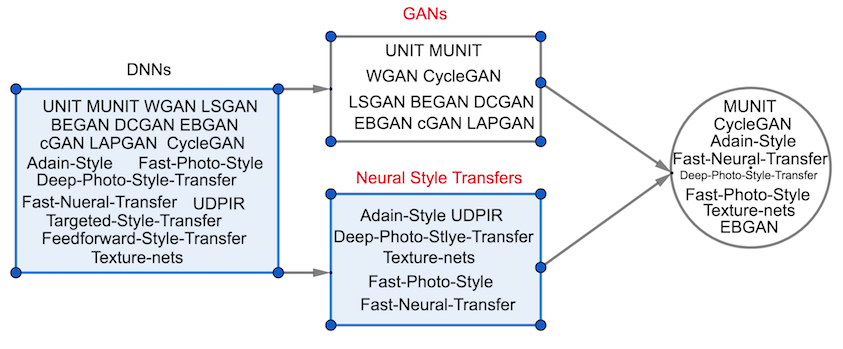
\includegraphics[width=0.9\textwidth]{filter}
    \caption{模型筛选过程}
    \label{fig:filtering}
\end{figure}

在有了足量的数据集后,基于DeepRoad的工作,我们首先选择实验的DNN模型大类是对抗生成网络\cite{GAN},因为其生成仿照数据的功能契合我们对于合成驾驶场景图片的需求,为了对目前所有的对抗生成网络技术能有一个综合的认识,我们首先参考了文献\cite{gan-survey},其中给出了目前学术界最为主流、为人熟知的几个模型算法:cGAN\cite{cGAN},DCGAN\cite{dcgan},LAPGAN\cite{LAPGAN}和EBGAN\cite{ebgan}等。我们一次对上述算法模型都进行了实验,但是其中dcGAN和LAPGAN在论文中没有开放其实验源码,且DCGAN在我们已有的路况图片数据集上的实验效果十分不理想,于是在实验初期我们排除了这几个模型。

在实验过上述模型后,我们通过Google搜索引擎,论文引用等途径陆续又发现了对抗生成网络中可以实现图像合成的几个模型,其中有一类是属于图片合成的输入需要有一张大致的纹理图,即给定一张样本纹理图和一组待转换的原图,输出为纹理跟输入纹理图一致的一组合成图,很明显这根我们的实验目的不匹配,因此被排除了。这一大类的模型有:MGAN\cite{MGAN},SGAN\cite{SGAN}和PSGAN\cite{PSGAN}。

另一类是属于图像填充功能,即跟据图片整体图像风格自动补充图片中因各种原因产生的空缺漏洞,这在计算机图形学和计算机视觉一致是个热门的研究领域,传统的方法是使用像素的复制和插值等数学方法来填充。对抗生成网络则提出了不一样的方法,通过学习大量同类的完整图片来实现图片的自动填充功能,比如文献\cite{GAN-inpaiting}提出的内容编码器方法。但由于这类模型跟我们图像风格转换的需求不匹配,因此没有做更深入的调研。

类似的,还有专门为人脸图像合成的模型,比如Age-cGAN\cite{Age-cGAN}。该类模型一般由一个编码器和条件对抗生成网络组成,其中编码器$E$将人脸图像$x$映射到一个潜在向量$z$中,条件生成器$G$在将潜在向量$z$和条件年龄变量$c$映射到合成一张新的人脸图。为了验证该类模型效果,我们首先在人脸数据上对这类模型进行了实验,成功复现了人脸自动合成的功能,但其在自动驾驶场景转换上的效果却很差。这可能是因为模型中使用的条件年龄变量对于自动驾驶场景图像的生成没有对应的参照物,因此这一类模型实验数据我们没有作最后的统计。


图\ref{fig:filtering}是我们对对抗生成网络模型筛选的大概历程,前后我们实验过的模型11个,最后统计实验数据统计总结的模型个数有4个,即UNIT\cite{UNIT},MUINT\cite{MUNIT},CycleGAN\cite{CycleGAN}和EBGAN\cite{ebgan}。

在选择对抗生成网络模型的过程中,除了模型本身的合成效果特点外,最大的困难是合适的数据集收集。在实验的初期我们就注意到大多数的对抗生成网络模型的训练都对其训练数据集有较为严格的要求,即需要训练集中的内容图片集和风格图像集尽可能的接近。

在调研了深度学习技术重点对抗生成网络大类后,我们重点参考了文献\cite{nst-survey},了解到目前能够实现图像转换技术的深度学习框架比较流行的还有一类叫做图像风格转换技术的框架,顺着文献的分类我们对立面提到的模型都实验了一遍。最开始我们选取的是比较有代表性的Fast Neural Transfer进行了实验,最终结果差强人意。由于正如文献中提到的,图像风格转换技术最初是为人工合成艺术作品而产生的一项深度学习技术,在我们对这类技术模型实验的过程中发现大多数模型实验的结果虽然可以实现图像的风格转换,但都太艺术化了,距真实场景的图片出入太大,所以大部分的模型的实验结果我们最后都排除在了统计范围内,最后作为数据统计的模型有:Adin-Style\cite{adain},Deep Photo Style Transfer\cite{dpst},Fast Photo Style\cite{fps},Fast Neural Transfer\cite{FNT}和Texture Nets\cite{texture-nets}。

% TODO 插入图片

以上是我们对实验模型筛选的大致历程,下面简单的介绍一下对抗生成网络的背景以及选择的对应模型。

\subsection{对抗生成网络大类}[Generative Adversarial Network Class]

对抗生成网络\cite{GAN}首先由Ian J. Goodfellow等人提出,它的本质是模拟真实数据源的概率分布。其基本框架有两个神经网络组成:生成模型网络和判别模型网络,其中判别模型负责学习区分数据是否来自真实数据分布,而生成模型可以想象成一个制造伪币的团伙,试图产生能够通过货币监测的钞票,判别模型正是这个对抗游戏中的警察,试图甄别出货币中的假钞。整个对抗生成网络模型的训练过程就是对抗模型和生成模型的训练竞赛,整个训练过程直到判别模型再也区分不出数据是来自真实数据分布还是生成模型伪造的数据为止。

训练过程中,对抗模型一般使用向后传播算法,而判别模型一般使用向前传播算法。其中判别模型为了通过数据$x$学习生成器的数据分布$p_g$,可以基于输入的噪声数据定义一个先验概率$p_z(z)$,然后将整个数据空间表示为$G(Z;\theta_g)$,这里的$G$是一个参数为$\theta$的多层神经网络可微函数。再定义一个输出为一个单向量的多层神经元网络$D(x;\theta_d)$,其中$D(x)$表示数据$x$来自真实数据而非$p_g$的概率。我们训练$D$直到我们对所有数据正确标记其是否来自判别器的概率最大为止。同时也训练$G$来最小化$\log(1-D(G(z)))$。上述可总结成下面的公式:
\begin{equation}
    \label{eq:gan}
    \min_G\max_DV(D,G)=\xi_{x\sim p_{data}(x)}[\log D(x)]+\xi_{z\sim p_z(z)}[\log(1-D(z))]
\end{equation}
实际训练过程中,等式\eqref{eq:gan}中的生成器$G$可能会出现梯度消失的问题,但由于本文章不是对对抗生成网络算法的研究,所以就不在此展开了。实验过程中为了保持尽量跟框架作者实现的效果性能一致,我们只选取了提供了源代码的框架进行了实验。

% TODO: confirm this
\textbf{统一说明},本文后续所有的实验均是在64位Ubuntu 16.04.6 LTS操作系统,8核GTX 1080ti-GPU硬件环境下进行的。以下介绍在本次实证研究中所有实验过用于图像风格转换的深度学习模型。

\subsubsection{cGAN}

\textbf{cGAN.}\cite{cGAN}\quad 对抗生成网络一般有两个对抗模型组成:一个可以捕捉到真实数据分布的生成模型$G$和一个能够计算样本来自训练数据集而不是$G$的概率的模型$D$。$D$和$G$都是非线性映射函数,比如多层感知器网络。如果生成器和判别器都限定于一些额外信息$y$上,则对抗生成网络可以被拓展成一个条件模型。其中$y$可以使任意类型的辅助信息,比如来自其他模型的数据或标记。cGAN通过将数据信息$y$送入判别器和生成器中作为额外的输入层来实现条件限制。在生成器中先验噪声输入$p_z(z)$和$y$被混合在联合隐藏层中,在判别器中$x$和$y$代表判别函数的输入,cGAN的目标函数可以表示为:
\begin{gather}
    min_G max_D V(D,G)=\mathbb{E}_{\x\sim p_{data}(x)}[\log D(x|y)]+\mathbb{E}_{z\sim p_z(z)}[\log(1-D(G(z|y)))]
\end{gather}

因为文献中\cite{cGAN}主要对MNIST\cite{mnist}数据集进行了数字模拟合成,在已有的路况图像数据集上实验的结果很不理想,且文献中提供的代码对数据集的要求也与一般的模型输入不一样,需要额外的处理,因而我们放弃了在该模型上的进一步实验与数据统计。 

\begin{figure}[h]
    \centering
    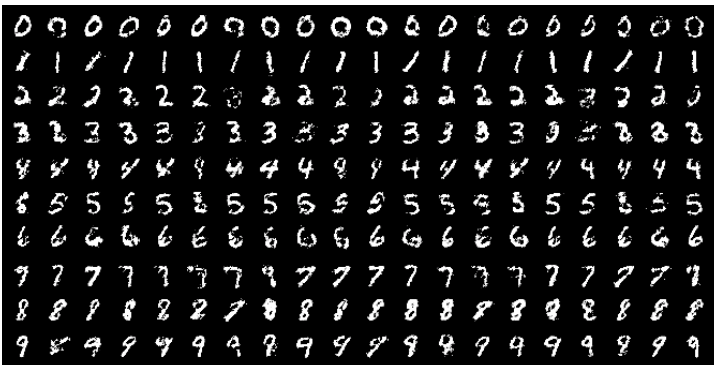
\includegraphics[width=.65\textwidth]{results/cgan}
    \caption{cGAN在MNIST数据集上的数字合成图片样例}
\end{figure}

\subsubsection{DCGAN}[DCGAN]

\textbf{DCGAN.}\cite{dcgan}\quad 是一个深度卷积对抗生成网络,其生成器和判别器使用的是限制卷积网络,主要的架构特点有:(1)用多步卷积和分布卷积层代替了所有的池化层(pooling layer);(2)使用了批量统一化层(batch normalization layer);(3)去掉了所有的全连接层;(4)在生成器中,使用$\tan{h}$作为输出层的激活函数,ReLU函数作为其它层的激活函数;(5)判别器中,所有层的激活函数都使用LeakyReLU函数。除此之外该算法结构中,所有正定空间池化函数都换成了多步卷积函数,这样可以使网络网络学习到整个图像空间的采样。

DCGAN主要目的是找到一个方法能够对图像进行特征重建及特征提取。DCGAN在其卷积神经网络的拓扑结构内提出了一套限制,使得该模型能够几乎在任何参数设置里都能够尽快的训练收敛。相较其他的对抗生成网络模型,DCGAN的主要优点是其稳定的网络结构和较快的训练收敛速度。DCGAN的作者将该模型在CIFAR-10\cite{cifar10}数据集上做了一次实证研究,结果也验证了DCGAN较其他GAN模型能够更快的学习到图像的特征。

虽然DCGAN的作者将其运用在人脸合成与转换上相当成功,但我们后来将其训练集换成了Udacity的自动驾驶路况数据集以及youtube上爬取的数据,实验结果样本图如下图\ref{dcgan_example}所示,效果却不理想。

\begin{figure}[h]
    \centering
    \subfigure[DCGAN在人脸图像合成的效果样例图]{
        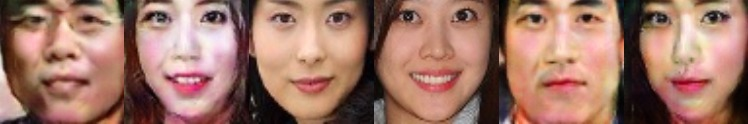
\includegraphics[width=0.75\textwidth]{dcgan_example}
    }
    \subfigure[DCGAN在自动驾驶数据集上的效果样例图]{
        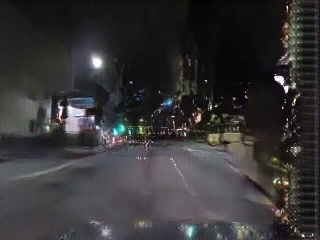
\includegraphics[width=0.4\textwidth]{results/dcgan_night}
        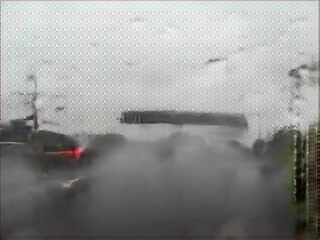
\includegraphics[width=0.4\textwidth]{results/dcgan_rain}
    }
    \caption{}
    \label{dcgan_example}
\end{figure}

实验代码使用的是\cite{dcgan}论文中给出的代码,其中主要参数配置如下

\begin{lstlisting}[basicstyle=\small]
    --bathSize     200          // 批量实验数据大小
    --imageSize    180, 320     // 设置图像尺寸大小
    --nz           20           // z向量
    --niter        10000        // 训练的次数
    --lr           0.0002       // Learning rate
    --cuda                      // 在cuda库上训练
\end{lstlisting}

由于DCGAN在驾驶路况图片上的合成效果很差,于是我们放弃了对该框架进一步的实验结果数据统计与总结。

\subsubsection{LAPGAN}

\newmodel{LAPGAN} 该模型利用了图像的多尺度结构,针对每个尺度构建了一系列的生成模型,每个模型都在特定尺度的拉普拉斯算子\cite{lapcode}上捕获到了图像的结构特征。这种方法将原来的图像转换问题成功地分解成了一系列可控状态,对于每个状态都可以使用一般的对抗生成网络结构训练一个基于卷积神经网络的生成模型。

在视觉应用,比如目标分类中的判别模型中,使用深度学习的方法常常十分有效。但是对于生成模型,尽管进行了相当多的研究\cite{lapgan1}\cite{lapgan2}\cite{lapgan3},却往往没有取得同等级别的成功。基于这样的问题,LAPGAN提出了模型在生成模型的训练效果上取得了巨大的改进。模型中使用的拉普拉斯算子是由一组图像的线性非可逆表征组成。具体的,使$d(\cdot)$表示模糊化$i\times j$图像$I$的缩减采样算子,则$d(I)$表示尺度为$j/2\times l/2$的新图像。类似地,令$u(\cdot)$表示将图像$I$光滑化的升采样算子,$u(I)$表示尺度为$2j\times 2j$的新图像。算法中首先构建一个高斯拉普拉斯算子$\mathbb{G}(I)=[I_0,I_1,\dots,I_K]$,这里的$I_0=I$和$I_k$表示$d(\cdot)$对$I$的$k$次重复操作。$K$是该算子中的层数。拉普拉斯网络中每一层$k$的系数$h_k$都是由邻近层中的距离计算构成,对图像使用算子$u(\cdot)$进行升采样操作:
\begin{gather}
    h_k=\mathbb{L}_k(I)=\mathbb{G}(I)-u(\mathbb{G}_{k+1}(I))=I_k-u(I_{k+1})
\end{gather}
每层都很直观的包含了特定尺度的图像结构信息。拉普拉斯算子$h_k$的最终结构是一张不同的图像。以此为基础可成功的重构一张新图像。

该算法文献\cite{LAPGAN}中在CIFAR10数据集上进行了图像转换实验,但实验的代码没有进行开源,因此我们暂时性的忽略了该算法的实验。将来该算法代码开源后我们会针对该算法进行补充实验和数据统计。 

% wc ~ 1200

\subsubsection{CycleGAN}[CycleGAN]

\textbf{CycleGAN.}\cite{CycleGAN}\quad 该模型的本质是学习不同图片类(比如晴天和雨天)的数据分布映射函数。给定两个不同类的数据集$X$和$Y$以及训练样本集$\{x_i\}_{x=1}^N, \{y_j\}_{j=1}^M$,其中$x_i\in X, y_j\in Y$。将数据分布记为$x\sim p_{data}(x), y\sim p_{data}(y)$。如图\ref{lable-cyclgan}所示,CycleGAN包含两个映射函数$G: X\to Y$和$F: Y\to X$,其次,CycleGAN还引进了两个判别器$D_X$和$D_Y$,其中$D_X$的目标是区分图像集$\{x\}$和转换的图像集$\{F(y)\}$,同样的,$D_Y$的目标是区分图像集$\{y\}$和$\{G(x)\}$。最终模型的训练目标是得到两个损失函数:(i)对抗损失函数,可以将合成的图像数据分布匹配对应到目标类的数据分布上;(ii)循环一致损失函数,阻止之前学习到的两个映射函数$G$和$F$彼此相矛盾。

\begin{figure}[h]
    \centering
    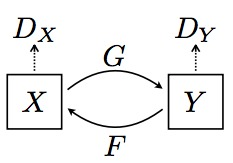
\includegraphics[width=.35\textwidth]{cyclegan_1}
    \caption{CycleGAN}
    \label{lable-cyclgan} 
\end{figure}

CycleGAN将对抗损失应用到了两个映射函数上,对于映射函数$G:X\to Y$和他的判别器$D_Y$,可以将其目标函数表示为
\begin{equation}
\begin{aligned}
    \label{eq:2}
    L_{GAN}(G,D_Y,X,Y)= & \xi_{y\sim p_{data}(y)}[\log D_Y(y)] + \\
    & \xi_{x\sim p_{data}(x)}[\log (1-D_Y(G(x)))]
\end{aligned}
\end{equation}

这里的$G$试图产生类似于类$Y$的图像集$G(x)$,然而$D_Y$的目标是区分转换的图像$G(x)$和真实的图像数据$y$。$G$旨在与对抗器$D$竞争最小化该目标函数。

\begin{figure}[b]
    \centering
    \subfigure[原始图片]{
        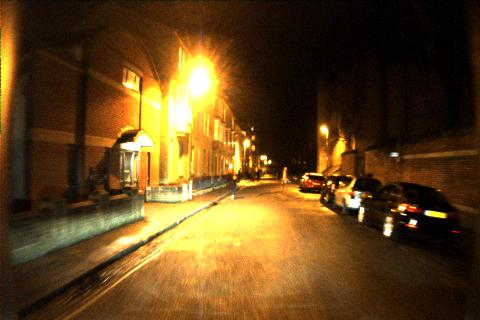
\includegraphics[width=0.3\textwidth]{results/cyclegan-input}
    }
    \subfigure[白天场景]{
        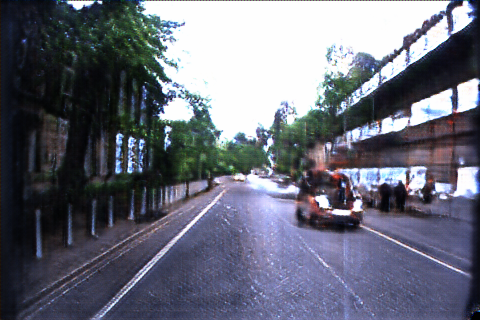
\includegraphics[width=0.3\textwidth]{results/cyclegan-sun}
    }
    \subfigure[黑天场景]{
        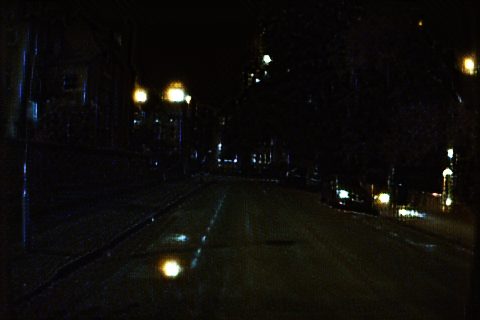
\includegraphics[width=0.3\textwidth]{results/cyclegan-night}
    }
    \subfigure[官方样例-1]{
        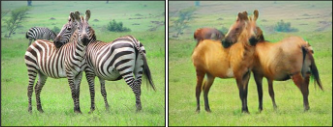
\includegraphics[width=0.45\textwidth]{cyclegan_o_1}
    }
    \subfigure[官方样例-2]{
        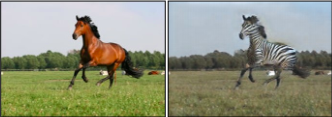
\includegraphics[width=0.45\textwidth]{cyclegan_o_2}
    }
    \caption{CycleGAN实验样例图以及官方图像转换样例图}
    \label{fig:cyclegan}
\end{figure}

对抗器理论上可以训练出可以输出和目标类$Y$与$X$分布完全相同的数据的映射函数$G$和$F$,但是如果网络的体积足够大,可以将相同的输入图片集映射到目标图片类的任意图像子集里。因此,单靠对抗损失函数无法保证学习到了映射函数能将单张输入图片$x_i$映射到理想的输出$y_i$。为了进一步减小可能的映射函数空间,CycleGAN提出循环一致映射函数,即对于来自类$X$的每张图像,对应的图像转换循环应该能够将$x$转换成原始图片,即\textit{向前循环一致}。上述的循环一致损失函数可以表示为:
\begin{equation}
\begin{aligned}
    \label{eq:3}
    L_{cyc}(G,F)= & \xi_{x\sim p_{data}(x)}[||F(G(x))-x||_1] + \\
    & \xi_{y\sim p_{data}(y)}[||G(F(y))-y||_1]
\end{aligned}
\end{equation}

综合等式\ref{eq:2}和等式\ref{eq:3}我们可以得到总的目标函数:
\begin{equation}
\begin{aligned}
    L(G, F, D_X, D_Y) = & L_{GAN}(G,D_Y, X, Y) \\
    & + L_{GAN}(F,D_X, Y, X) \\
    & + \lambda L_{cyc}(G, F)
\end{aligned}
\end{equation}
这里的$\lambda$控制着两个目标的相对重要性。

CycleGAN对于内容图片通训练图片不相似的情况转换合成效果并不好,常常会造成合成图的语义不明确。它通常适合于颜色和图像纹理转换的情形,对于合成图有内容变化的情形,CycleGAN合成图的效果会比较差,其作者分析其中的原因可能是因为常常会为了提高图像信息变化更高效而裁减生成器的网络复杂度,这使得CycleGAN对于内容改变的性能变差。文献\cite{CycleGAN}中也提到了CycleGAN对于一组不相似的图片训练出来的模型效果较一组相近训练数据集模型效果会差很多,并且很难消除这两者间的差异。

图\ref{fig:cyclegan}是我们将CycleGAN运用在我们的数据集上,进行了晚上到白天以及黑天场景转换的实验结果样本图以及CycleGAN在其官方给定的数据集上的图像转换效果。 

% wc ~ 800

\subsubsection{WGAN}

\newmodel{WGAN} 该算法相较其他的GAN模型的主要改进依然是提升了模型训练的稳定性和收敛速度。WGAN提出了Earth-Mover距离,并证明了该距离比其他的距离尺度指标能产生更好的梯度,从而提升训练速度。此外它关于判别器网络还去掉了对应了sigmoid层,在对抗损失函数中去掉了log函数,有效地避免的类似模型塌缩等问题。理论上图像合成的效果要好于DCGAN。

因为WGAN文献中只给出了算法的核心思想,没有给出实验源码。我们参考文献中提供的算法,实现了WGAN的图像转换代码,但是在路况图像数据集上的实验结果十分不理想,合成的图像与原图像在语义上相差甚远,我们猜测可能是算法实现没有成功导致,最终我们没有将该实验结果纳入最后的实验数据总结和统计中。

\subsubsection{MUNIT}[MUNIT]

\textbf{MUNIT.}\cite{MUNIT}\quad MUNIT是基于UNIT\cite{UNIT}工作的进一步优化。它主要针对的问题时候多类图像间的图像转换问题。比如一个冬天的道路场景在夏天可能会依天气、时间等因素的不同而有很多种不同的外在形式。CycleGAN希望其生成器能够包含一个场景中尽可能多的表征空间。

除此之外它提出了一个可以解决多模型图片到图片转换问题的框架。它对于图像转换问题提出了几个假设:图片的潜在空间(latent space)可以被分解成内容空间和样式空间。基于上一个假设又提出了不同域类的图片共享一个类似的内容空间,但样式空间不一致。为了将一张图片转换成目标域类,MUNIT提出可以将图片的内容码与目标域类样式码空间的一个随机样式码重组。这里的内容码代表了在图片转换过程中应该被保留的信息元,而状态码则代表了不包含在输入图片中还剩下的变量元。通过采样不同的状态码,MUNIT模型能够产生多样,多模型的输出。以上严格的数学定义如下:

\begin{figure}[t]
    \centering
    \subfigure[原始图片]{
        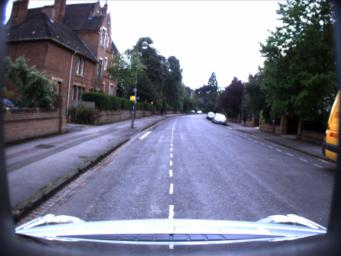
\includegraphics[width=.3\textwidth]{results/munit}
    }
    \subfigure[雪天场景1]{
        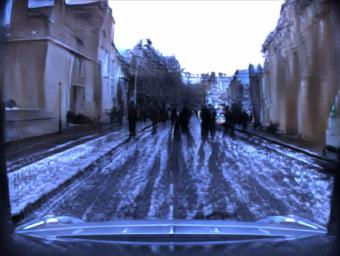
\includegraphics[width=.3\textwidth]{results/munit_winter}
    }
    \subfigure[雪天场景2]{
        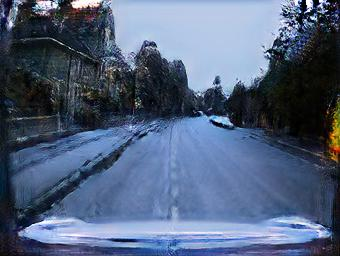
\includegraphics[width=.3\textwidth]{results/munit_winter2}
    }
    \subfigure[官方实验样例图]{
        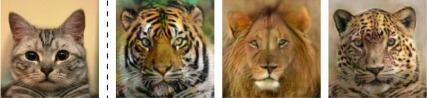
\includegraphics[width=0.8\textwidth]{munit_o_1}
    }
    \caption{MUNIT实验样例图}
    \label{fig:munit}
\end{figure}

假定$x_1\in \chi_1$和$x_2\in \chi_2$是来自两个图片域类的图片集,给定来自两个不同边缘分布$p(x_1)$和$p(x_2)$的样本图片集,但不知道联合分布$p(x_1, x_2)$。MUNIT的目的是利用学习到的图片到图片转换模型$p(x_{1\to 2}|x_1)$和$p(x_{2\to 1}|x_2)$来预测两个边缘分布$p(x_1|x_2)$和$p(x_2|x_1)$,这里的$x_{1\to 2}$是由将$x_1$转换成$x_2$产生的一个样本输出。一般来说,$p(x_1|x_2)$和$p(x_2|x_1)$通常是十分复杂且多模型分布,为了简化这两个边缘分布,MUNIT提出了\textit{部分共享潜在空间假设}。即假设每张图片$x_i\in \chi_i$都是由两种码,内容码和样式码,组成,其中内容码$c\in C$由两个类域共享,而样式码$s_i\in S_i$则是每个域类图片所特有的。换句话说,一组来自联合分布的对应的图片$(x_1, x_2)$是由$x_!=G_1^*(c,s_1)$和$x_2=G_2^*(c, s_2)$生成的,这里的$c,s_1,s_2$都是来自鲜艳分布,$G_1^*,G_2^*$是实际的生成器。进一步假设$G_1^*$和$G_2^*$是确定性函数,且有反解码器$E_1^*=(G_1^*)^{-1}$和$E_2^*=(G_2^*)^{-1}$。MUNIT的目的是利用神经网络学习实际的生成器以及编码函数。它使用了两个重建的目标函数:给定来自数据分布的图像样本,在编码和解码后我们能够重建它:
\begin{gather}
    L_{recon}^{x_1}=E_{x_1\sim o(x_1)}[||G_1(E_1^c(x_1), E_1^s(x_1))-x_1||_1] 
\end{gather}

给定在转换时的样式和内容码,我们也应该能够在解码和编码后重建图像:
\begin{equation}
    \begin{aligned}
        L_{recon}^{c_1}= & E_{c_1\sim p(c_1), s_2\sim q(s_2)}[||E_2^c(G_2(c_1,s_2))-c_1||_1] \\
    L_{recon}^{s_2}= & E_{c_1\sim p(c_1), s_2\sim q(s_2)}[||E_2^s(G_2(c_1, s_2))-s_2||_1]
    \end{aligned}
\end{equation}

结合以上公式,MUNIT的总的损失函数可以由下面的公式表示:
\begin{equation}
\begin{aligned}
    \min_{E_1,E_2,G_1,G_2}\max_{D_1,D_2}L(E_1,E_2,G_1,G_2,D_1,D_2)=L_{GAN}^{x_1}_L_{GAN}^{x_2}+\\
\lambda_x(L_{recon}^{x_1}+L_{recon}^{x_2})+\lambda_c(L_{recon}^{c_1}+L_{recon}^{c_2})+\lambda_s(L_{recon}^{s_1}+L_{recon}^{s_2})
\end{aligned}
\end{equation}

总体来说,MUNIT是一个多模型无监督图像到图像的转换框架。在目前的无监督方法中图像转换质量和转换图像的种类都更好更多。最后我们使用了MUNIT提供的代码,进行了晴天路况图和雪天场景的转换,主要的优化配置参数如下,最终的实验结果样例及MUNIT官方实验样例图参考图\ref{fig:munit}:

\begin{lstlisting}[basicstyle=\small, caption={MUNIT主要优化参数配置}, captionpos=b]
    max_iter: 1000000             # maximum number of training iterations
    batch_size: 1                 # batch size
    weight_decay: 0.0001          # weight decay
    beta1: 0.5                    # Adam parameter
    beta2: 0.999                  # Adam parameter
    init: kaiming                 # initialization [gaussian/kaiming/xavier/orthogonal]
    lr: 0.0001                    # initial learning rate
    lr_policy: step               # learning rate scheduler
    step_size: 100000             # how often to decay learning rate
    gamma: 0.5                    # how much to decay learning rate
    gan_w: 1                      # weight of adversarial loss
    recon_x_w: 10                 # weight of image reconstruction loss
    recon_s_w: 1                  # weight of style reconstruction loss
    recon_c_w: 1                  # weight of content reconstruction loss
    recon_x_cyc_w: 10             # weight of explicit style augmented cycle consistency loss
    vgg_w: 0                      # weight of domain-invariant perceptual loss
\end{lstlisting}

\subsubsection[EBGAN]{EBGAN}

\begin{figure}[b]
    \centering
    \subfigure[原始图片]{
        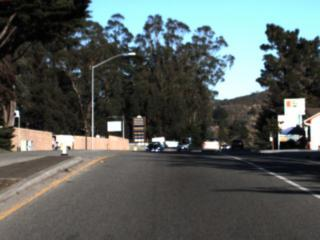
\includegraphics[width=.45\textwidth]{results/ebgan-input}
    }
    \subfigure[雨天场景]{
        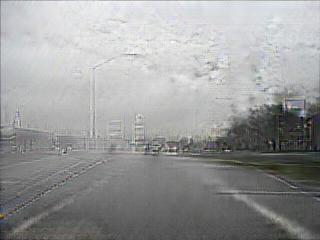
\includegraphics[width=.45\textwidth]{results/ebgan-rain}
    }
    \subfigure[官方人脸合成样例图]{
        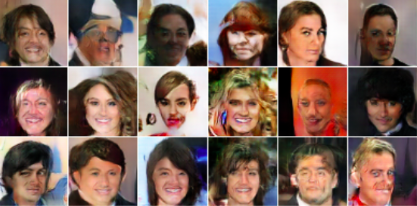
\includegraphics[width=0.8\textwidth]{ebgan_o_1}
    }
    \caption{EBGAN实验样例图}
    \label{fig:ebgan}
\end{figure}

\textbf{EBGAN.}\cite{ebgan}\quad 的核心思想是将判别器视为一个能量函数而不是通常的概率函数。它构建了一个函数能将输入空间中的每个点映射成为一个单标量,并且提出了对抗生成模型训练的一个基于能量表达的公式。由判别器计算出来的能量函数可以被视作生成器的可训练代价函数。虽然可以将能量函数通过Gibbs分布转换成概率函数,但是基于它提出的基于能量形式的对抗生成网络由于缺少归一化,从而使我们在判别器的架构和训练过程中有了更多的选择。EBGAN的学习构成是由数据驱动,定型能量函数是的好的模型参数配置获得低能量而不好的配置参数获得高能量。这种训练书序监督学习的一种:对于每训练集中的每个$X$,一种$(X,Y)$的能量只有当$Y$是好的配置参数时才会获得低能量,反之获得高能量。下面简单阐述一下EBGAN的基本原理。

将$p_{data}$视作产生真实数据集分布的概率密度函数,生成器$G$训练生成赝本数据$G(z)$。为了定义能量函数,判别器的输出通过一个目标泛函算子进行转换,将低能量视为真实样本数据,而高能量则为合成的伪数据。跟一般的对抗生成网络一样,EBGAN也使用了两个不同的损失函数来分别训练生成器和判别器。

给定一个正边缘分布函数$m$,一个数据样本$x$和一个生成样本$G(z)$,判别器损失函数$L_D$和生成器损失函数$L_G$可以定义为以下:
\begin{equation}
    \begin{align*}
    L_D(x, z) = & D(x) + [m - D(G(z))] \\
    L_G(z) = & D(G(z))
    \end{align*}
\end{equation}

给定一个生成器$G$,$p_G$为$G(z)$的密度分布,这里$z\sim p_z$。换句话说,$p_G$是由$G$产生的样本的概率密度函数。定义$V(G,D)=\int_{x,z}L_D(x,z)p_{data}(x)p_z(z)dxdz$和$U(G,D)=\int_zL_G(z)p_z(z)dz$,训练中判别器来最小化$V$值,生成器最小化$U$值。该系统的纳什均衡是一组满足一下条件的一对$(G^*,D^*)$:
\begin{equation}
    \begin{aligned}
        V(G^*,D^*) \leq V(G^*,D) \quad\quad \forall D \\
        U(G^*,D^*) \leq U(G,D^*) \quad\quad \forall G 
    \end{aligned}
\end{equation}

EBGAN打通了两类不同的非监督学习方法:对抗生成网络和自动编码器,并且从基于能量的角度重新采用对抗生成网络的结构并定义新的训练损失函数。对于高分辨率图片,相较其他类的对抗生成网络技术,EBGAN的模型训练有更快的收敛速度,且合成图片也有更好的合成效果。

我们在已有的数据集上使用了tensorflow实现的EBGAN代码\cite{ebgan-github},实现了晴天路况到雨天场景的转换,图\ref{fig:ebgan}是实验结果样例图及官方人脸合成实验样例图。

\subsubsection{LSGAN}

\newmodel{LSGAN} 一般的GAN模型都使用sigmoid交差熵作为判别器的损失函数,使用这类损失函数都存在一个问题,就是在模型训练过程中很容易出现梯度消失的问题,导致最后合成的数据离真实数据分布相差较大。针对这一问题LSGAN提出使用最小方差函数最为判别器的损失函数,因为最小方差损失函数能够使判别器对接近判断边界的伪数据做出惩罚。除此之外,LSGAN还能提高模型训练过程的稳定性。文献\cite{LSGAN}提到实验结果显示LSGAN合成的数据别一般的GAN合成输数据更接近与真实数据分布。该算法的目标损失函数为:
\begin{equation}
\begin{aligned}
    & \min_D V_{LSGAN}(D)=\frac{1}{2}\mathbb{E}_{x\sim p_{data}(x)}[(D(x)-b)^2]+\frac{1}{2}\mathb{E}_{z\sim o_z(z)}[(D(G(z))-z)^2] \\
    & \min_G V_{LSGAN}(G)=\frac{1}{2}\mathb{E}_{z\sim p_z{z}}[(D(G(z))-c)^2]
\end{aligned}
\end{equation}

下图\ref{fig:lsgan}是LSGAN和一般的GAN图像合成样本的对比图。

\begin{figure}[h]
    \centering
    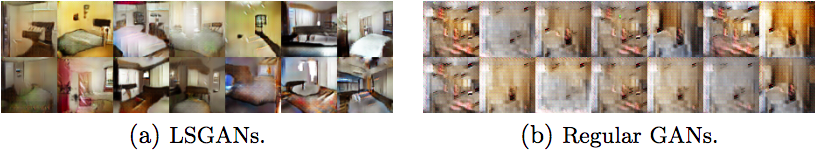
\includegraphics[width=\textwidth]{results/lsgan}
    \caption{LSGAN合成图像对比图}
    \label{fig:lsgan}
\end{figure}

由于文献中的实验代码没有开源,于是我们利用DCGAN的源码将其判别器的损失函数改为文献中提到了最小方差函数,但是最后的实验结果跟DCGAN的实验结果相差不大。基于较差的实验结果我们舍弃了该模型实验结果的数据统计和总结。

\subsubsection{MGAN}

\newmodel{MGAN} 大部分用于图像合成的对抗生成网络技术都是使用马尔可夫随机场来处理图像复杂的限制特征,这些马尔可夫随机场也通常是使用像素块的统计数据来表征图像的。这类技术通常分为两类:合成完整图像的全图像模型和只合成图像纹理层的马尔科夫模型。MGAN主要的改进是提升了深度马尔科夫模型对纹理合成的效率与质量。文献\cite{MGAN}中使用对抗训练\cite{adtrain}算法训练卷积神经网络,这样可以维持与原图几乎不变的图片质量,同时极大地提升了图像合成速度,40ms内合成一张$512\times 512$图像,其中硬件条件为TitanX GPU。

因为MGAN的优化主要针对人脸合成类别,且与传统的图像合成技术类似,合成图片具有明显的艺术风格。我们利用文献中提供的代码\cite{git:mgan}在我们的路况图像数据集上实验结果跟文献中的实验结果一致,具有太明显的艺术风格,因而在最后的实验数据统计和总结环节我们没有考虑该模型的实验数据。下图\ref{fig:mag}为MGAN的实验数据样例图。

\begin{figure}[h] 
    \centering
    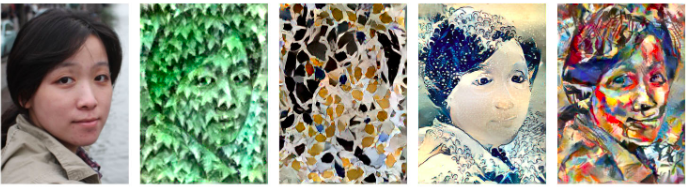
\includegraphics[width=.9\textwidth]{results/mgan}
    \caption{MGAN实验样例图}
    \label{fig:mag}
\end{figure}

\subsubsection{BEGAN}

\newmodel{BEGAN}  该模型跟EBGAN\cite{ebgan}一样使用了自动编码器作为判别器。虽然一般典型的对抗生成网络模型都直接匹配数据分布,但是BEGAN的目的是利用从Wasserstein距离中推到出了损失函数,来匹配自动编码器损失值。分布。实际的模型算法中,使用了一个典型的对抗生成网络目标函数,加上一个额外的平衡判别器和生成器的平衡因子。这样使得模型的训练更加容易。文献\cite{BEGAN}中对于自动编码器使用的损失函数$\mathb{L}:\mathbb{R}^{N_x}\to \mathbb{R}^+$为:
\begin{align}
    \mathb{L}(v) = |v-D(v)|^\eta where \begin{cases}
        D: \mathbb{R}^{N_x}\to \mathbb{R}^{N_x} \quad  \\
        \eta \in \{1,2\} \quad  \\
        v \in \mathbb{R}^{N_x} 
    \end{cases}
\end{align}

模型总体的目标函数可表示为:

\begin{align}
    \begin{cases}
        L_D = L(x) - k_t\cdotL(G(z_D)) & for \quad \theta_D \\
        L_G = L(G(z_G)) & for \quad \theta_G \\
        k_{t+1} = k_t + \lambda_k(\gammaL(x)-L(G(z_G))) 
    \end{cases}  
\end{align}

我们参照文献中的代码实现了WGAN的人脸图像合成,但将数据源换成我们的路况图像数据集后,程序出现了未知的BUG,导致最终的路况图像合成实验没能完成。下图\ref{fig:began}为BEGAN的人脸合成结果样例图。

\begin{figure}[h]
    \centering
    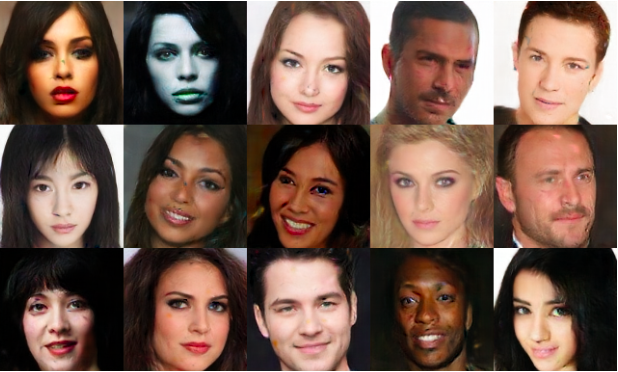
\includegraphics[width = .8\textwidth]{results/began}
    \caption{BEGAN人脸合成样例图}
    \label{fig:began}
\end{figure}

% wc ~ 1700

\subsection{图像风格转换大类}[Neural Style Transfer Class]

图像风格转换技术是受启发于近20年来卷及网络神经的发展,Gatys等人\cite{nst}提出利用卷积神经网络来复现一些著名的绘画风格。他提出利用神经元来实现将图像中的内容和风格分开和重组的功能。以物体识别中的卷积神经网络为例,其在训练过程中,会随着网络层数的增加,其神经元对图像表征能力也会随之增加。因此,随着网络结构层数的深入,输入图片也会被转换成比原始图中像素值更具表征性的神经元输出。于是Gatys提出可以直接从高特征层包含的信息重建图像。越高的网络层能够捕获更高级的图像语义信息。因此Gatys将高层中的特征表示看做图像的内容表征。

为了能将包含在网络结构中不同层间冬天图片信息可视化,文献\cite{nst}提出可以在一张白噪声图片上利用梯度下降算法来找到另一张可以匹配原始图片特征空间的图片。令$\overrightarrow{p}$和$\overrightarrow{x}$表示原始图片和合成图片。$P^l$和$F^l$分别表示它们在$l$层的表征。定义两个表征之间的方差损失为:
\begin{align}
    L_{content}(\overrightarrow{p},\overrightarrow{x},l)=\frac{1}{2}\sum_{i,j}(F_{ij}^l-P_{ij}^l)^2
\end{align}
该损失函数对应于$l$层激活函数的导数等于
\begin{align}
    \frac{\partial L_{content}}{\partial F_{ij}^l} = \begin{cases}
        (F^l-P^l)_{ij}  & if \quad F_{ij} > 0 \\
        0 & if \quad F_{ij}^l \lt 0
    \end{cases}
\end{align}

由此对用与图片$\vec{x}$的导数可以通过标准误差的向后传播算法计算得出,从而我们可以改变初始的随机图片$\vec{x}$直到在卷积层中某一层产生跟原始图$\vec{p}$表征一致的特征。

对于输入图像的风格表征,Gaatys利用原本用来捕获图像纹理信息的特征空间。该特征空间建立在网络层的过滤网之上。它由特征空间中不同层的过滤网之间的协方差组成,通过包含多层间的特征协方差,就可以获得一个静态、多尺度的输入图片表征值,该表征形式捕获了输入图像的纹理信息。

为了获得输入图片的风格表征形式,他们使用了一个原本用来获取图层信息的特征空间。该特征空间构建于神经网络的每一层过滤网之上。它由特征图谱各个部分的过滤网之间的协方差组成。通过引进多层网络之间的特征协方差,可以得到一个输入图片的一个静止、多尺度的能够包含图层信息的表征形式。再者,还可以通过构建一张匹配给定的输入图片的样式表达的图片来将建立在网络中不同层的样式特征空间信息可视化。为了合成拥有输入图片样式的图片,一般的图像风格转换技术会最小化来自一层网络的内容表征的白噪声图片与卷积网络层中输入图片的样式表征之间的距离。让$\overrightarrow{p}$表示合成照片,$\overrightarrow{a}$表示输入图片,则损失函数可以表示为:
\begin{align}
    L_{total}(\overrightarrow{p},\overrightarrow{a}, \overrightarrow{x})=
    \alpha L_{content}(\overrightarrow{p}, \overrightarrow{x}) +
    \beta L_{style}(\overrightarrow{a}, \overrightarrow{x})
\end{align}

这里的$\alpha$和$\beta$分别表示内容和样式在重建过程中的权重。一般地通俗来讲,Neural Style Transfer转换合成图片需要3张图片,即内容图片,风格图片(通常为艺术画等),及需要进行风格转换的输入图片。进行图像合成转换的原理即定义两个距离函数:$Lcontent$表示两张图片内容的差异,$Lstyle$表示两张图片就风格而已之间的差异。对于第三章输入图片,通过神经网络变换输入图片的像素值,使其内容同内容图片的距离最小化,风格同风格图片的距离最小化,最终的损失函数记为以上两个距离函数之和。 

下面我们参考了文献\cite{nst-survey},根据里面给出的分类抽取了具有代表性的几个模型进行了实验,实验平台跟之前的实验一致。

\subsubsection[AdaIN-style]{AdaIN-style}

\textbf{AdaIN-style.}\cite{adain}\quad AdaIN Style主要针对Gatys提出的Neural Style Transer算法中,模型的训练需要一个很慢的迭代优化算法,这大大延长了模型的训练时间,其限制了它在很多场景下的实用价值。因此AdaIN Style提出使用前向传播神经网络的快速逼近算法来加速图像风格转换技术。但是速度的提升也会导致网络限制在了固定的一套风格集中,而无法使用到任意的风格集中。针对以上问题AdaIN Style提出了可以实时转换任意风格的框架。

\begin{figure}[!hb]
    \centering
    \subfigure[]{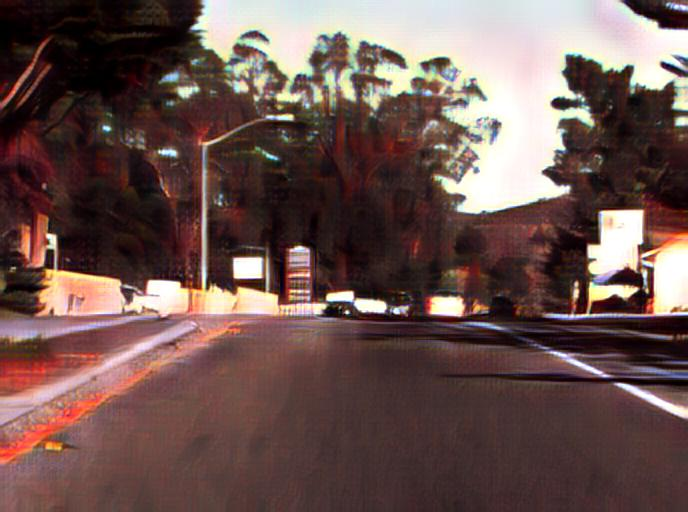
\includegraphics[width=.23\textwidth]{adin/adin1}}
    \subfigure[]{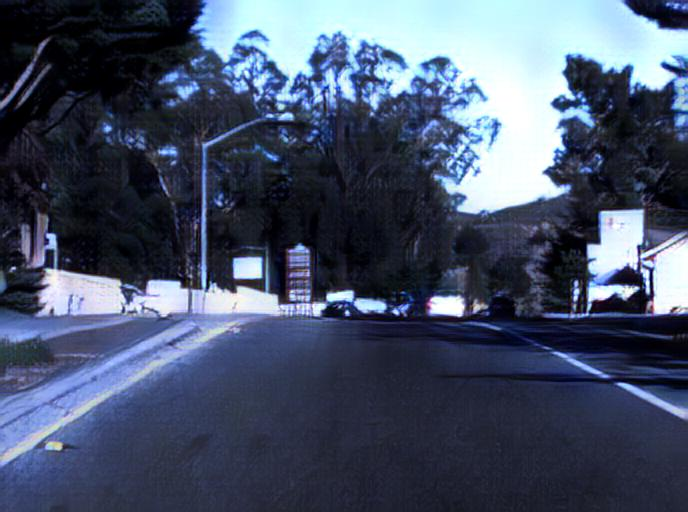
\includegraphics[width=.23\textwidth]{adin/adin2}}
    \subfigure[]{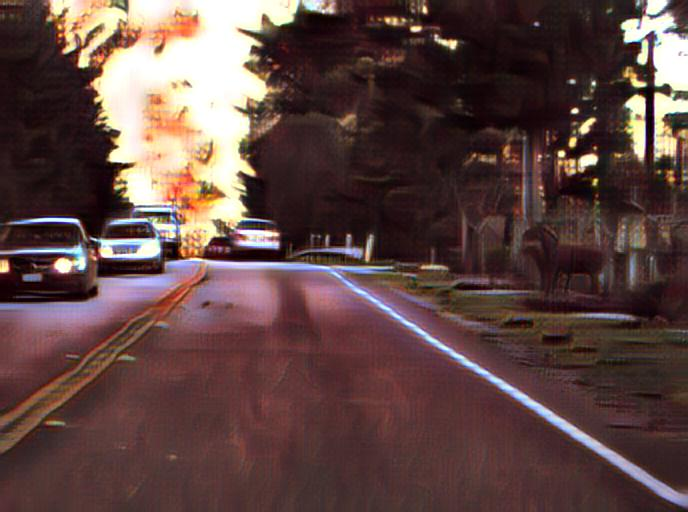
\includegraphics[width=.23\textwidth]{adin/adin3}}
    \subfigure[]{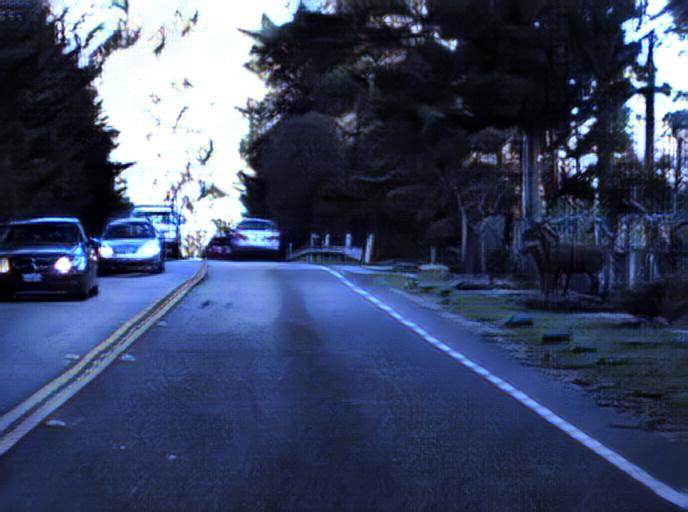
\includegraphics[width=.23\textwidth]{adin/adin4}}
    \subfigure[官方样例图]{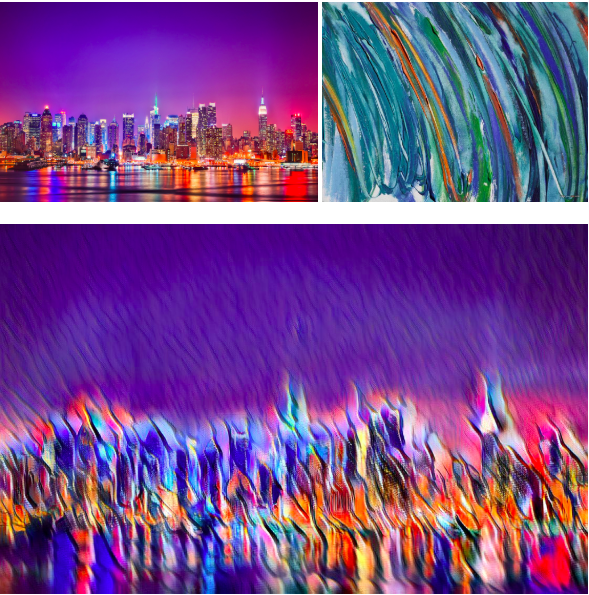
\includegraphics[width=.8\textwidth]{adin_o_1}}
    \caption{AdaIN实验结果样例图}
    \label{fig:adin}
\end{figure}

文献\cite{ioffe}提出批量正则化层极大的简化了向前传播网络的训练,AdaIN-style的模型结构也使用了批量正则化层,并且在次基础上通过将该层的激活函数改为单例正则,训练性能得到的巨大提升:
\begin{align}
    IN(x)=\gamma(\frac{x-\mu(x)}{\tau(x)})+\beta
\end{align}
与之前的批量正则层不同的是单例层在测试阶段不变,然而批量正则层通常会用总体统计数据替换掉批量神经元的均值。

除了学习仿射参数$\gamma$和$\beta$,另一个改进方式是为每一个样式$s$学习不同的参数$\gamma^*$和$\beta^*$:
\begin{align}
    CIN(x;s)=\gamma^*(\frac{x-\mu(x)}{\tau(x)})+\beta^*
\end{align}
训练过程中,样例图片和它的指数$s$被随机从一个固定的样例集合$s\in {1,2,\dots,S}(S=32)$选取。内容图片会被样式转换网络进行转换,该网络中对应的$\gamma^*$和$\beta^*$被用在条件单例正则层里。

总体来说,AdaIN通过转换特征统计量,特别是像素均值和方差,来实现特征空间的样式转换。除此之外,AdaIN Style加深了深度图像表征的理解。其与Gatys提出的Neural Style Transfer主要区别在于两者之间的优化过程和具体的优化函数的不同,AdaIN Style的网络结构也可以多变,而不局限于卷积神经网络一种。此外AdaIN Style相较于Gatys等人提出的原始算法,其算法图像合成速度在原来的基础上有近720倍的提升\cite{adin-github},且没有任何性能上的损失。在具体的风格转换实现中,该算法也提供了可以在多种风格之间以权值相加的方式融合新的风格的方法。算法中使用的网络模型是基于MSCOCO\cite{mscoco}数据集训练的。
AdaIN在已有的数据集上晴天转雪天、晚上的实验结果样例图以及官方的庚哥转换实验样例图\ref{fig:adin}。

% wc ~ 800

\subsubsection{Deep Photo Style Transfer}[Deep Photo Style Transfer]

\textbf{Deep Photo Style Transfer.}\cite{dpst}\quad  一般的基于Gatys等人提出的图像风格转换类似的技术都是对艺术品图像进行转换的技术,Deep Photo Style Transfer则主要针对的是显示中照片风格的转换。它主要的改进是限制了从输入图片到输出图片之间的变换为色彩空间的局部仿射变换,并且将该限制表示成了一个可自定义完全可微的能量函数。该方法可以成功地抑制合成图片中扭曲的现象。此外文献\cite{dpst}中还比较了该方法和Neural Style Transfer技术之间的转换效果,结果显示在后者出现的艺术效果以及图像中的边界扭曲效果都不存在于Deep Photo Style Transfer的合成图片中。跟之前的风格转移技术类似,也是基于将网络结构中不同层视为包含图像的内容信息和样式信息。下面简单介绍一下该技术的基本原理。

该算法不像之前的图像风格迁移技术,每次转换的输入为两组图像集合。该算法的输入仅为两张图片,与之前的一样分别为待转换的内容图片和参考的风格图片,模型的目的在于将风格图片中的风格迁移到内容图片中同时保留内容图片中的图像场景。另外该算法的一个优点是其风格图像中的Gram矩阵是基于整张图片计算的,它隐式的包含了模型中各个神经元信息,同时也限制了其分割语义图中各部分分割线的扩张。为了解决这个问题,该算法添加了为每张输入图片添加了对应的分割掩图来协助转换过程中语义分割部分转换的精确性。这些掩图被添加到原图上作为额外的通道,加上下面的分割通道来更新其风格损失函数,从而增强神经元风格算法:
\begin{equation}
    \begin{aligned}
    L_{s+}^l=\sum_{c=1}^C \frac{1}{2N_{l,c}^2}\sum_{ij}(G_{l,c}[O]-G_{l,c}[S])_{ij}^2\\
    F_{l,c}[O]=F_l[O]M_{l,c}[I]\quad F_{l,c}[S]=F_l[S]M_{l,c}[S] 
    \end{aligned}
\end{equation}
这里的$C$是语义分割掩图中的通道个数,$M_{l,c}[\cdot]$记为网络层$l$中分割掩图中的通道$c$,$G_{j,c}[\cdot]$表示对用的$F_{l,c}[\cdot]$中的Gram矩阵。为了匹配卷积神经网络中每层网络中的特征扩张空间,该算法降低了掩图的采样频率。

为了避免只出现在输入图像中的“孤独语义标记”,算法将输入的语义标记限制在了参考风格图像标记中。然而这样做可能对导致在参考样式图像上的错误标记,标记语可能在语义上大致是相同的,比如“江”和“湖”等。算法将3个部分组合形成了图像风格转换的目标函数:
\begin{align}
    L_{total}=\sum_{t=1}^L\alpha_lL_C^l+\Gamma\sum_{l=1}^L \beta_lL_{s+}^l +\lambda L_m
\end{align}
这里的$L$是卷积层的层数,$l$表示深度神经网络中的第$l$层。$\Gamma$是控制样式损失函数的权值,$\alpha_l$和$\beta_l$是调试层权重的参数。

Deep Photo Style Transfer也使用了提前训练好的VGG-19\cite{vgg-19}网络作为特征提取器,选用$conv4\_2$作为内容表征,$conv1\_1,conv2\_1,conv3\_1,conv4\_1$和$conv5\_1$作为风格表征,使用参数$\Gamma=10^2,\lambda=10^4$作为所有结果的偏好参数。

由于该模型中实现图片转换需要用到每张图片的语义分割掩图,文献\cite{dpst}中并没有给出生成掩图的代码,目前生成掩图且带有标注功能的开源工具都是基于人工对单张图片进行操作的,故而具体到我们实验的需求,对几万张Udacity数据集进行标注和语义分割,代价太大,因此我们只选用了部分数据集对该模型进行实验和结果统计。图\ref{fig:dps}是Deep Photo Style Transfer官方风格转换合成效果样例图。

\begin{figure}[h]
    \centering
    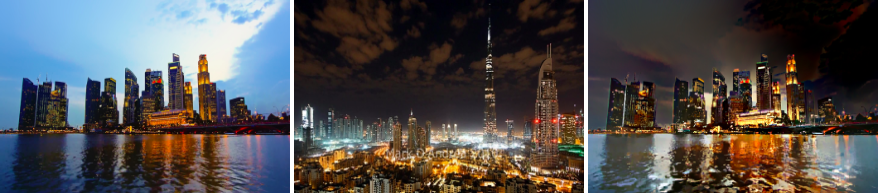
\includegraphics[width=.85\textwidth]{dps_o_1}
    \caption{Deep Photo Style Transfer官方实验样例图}
    \label{fig:dps}
\end{figure}

% wc ~ 1000

\subsubsection{Fast Photo Style}[Fast Photo Style]

\textbf{Fast Photo Style.}\cite{fps}\quad  提到其他的风格转换技术中存在的问题:合成的图片往往会有不一致的风格特征,且有比较明显不真实部分。这也是该算法主要希望解决的问题。此外,算法也希望最后合成的图片应该跟用相机拍摄的照片一样真实,相较其他的主要基于色调匹配来风格化图片的技术,不同的是Fast Photo Style还关注输入图像中个内容特征的学习与提取。

\begin{figure}[t]
    \centering
    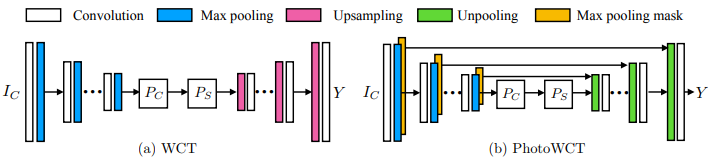
\includegraphics[width=.8\textwidth]{wct}
    \caption{}
    \label{wctf}
\end{figure}

该算法的风格化主要由两个关键步骤组成。第一步是名为PhotoWCT的样式转换$F_1$。给定一个样式图片$I_S$,$F_1$将$I_S$的风格迁移到内容图片$I_C$上,同时最小化最后的输出图片中的结构变化。虽然$F_1$可以很好的样式化$I_C$,但在语义上比较相近的区域上经常会合成样式不一致的图片。因此该算法使用了一个光滑函数$F_2$,试图借此来消除这些“坏掉的”部分。算法整体可以表达成下面的两步映射函数:
\begin{align}
    F_2(F_1(I_C,I_S),I_C)
\end{align}

PhotoWCT是基于WCT\cite{wctp}算法,为了实现真实的图片样式合成,它使用了一个新奇的网络架构。为了使用WCT,对于一般的图片重建的自动编码器被首先训练。一般的训练过程使用的是VGG-19模型作为编码器\varepsilon,并且训练解码器$D$来重建输入图片。解码器和编码器行程对称,在行为上互为逆反操作。当自动编码器训练好了,一堆映射函数就被插入到网络中,通过白化($P_C$)和彩色花($P_S$)变换来行使样式化操作。主要思想是通过两个映射函数直接将内容图像的特征相关映射到样式图片中。具体地,给定一堆内容图片$I_C$和样式图片$I_S$,首先提取除向量化的VGG特征$H_C=\varepsilon(I_C)$和$H_S=\varepsilon(I_S)$,然后再通过下面公司来转换内容特征$H_C$:
\begin{align}
    H_{CS}=P_SP_CH_C
\end{align}
这里$P_C=E_C\Lambda_C^{-\frac{1}{2}}E_C^T$,$P_S=E_S\Lambda_S^{\frac{1}{2}}E_S^T$,其中$\Lambda_C$和$\Lambda_S$是堆成三角矩阵,且有相同的协方差矩阵$H_CH_C^T$和$H_SH_S^T$。矩阵$E_C$和$E_S$是各自对用的特征向量的正交矩阵。转换后,特征方差会匹配样例图片的特征空间,即$H_{CS}H_{CS}^T=H_SH_S^T$。最后样例图片可以通过直接将转换后的特征映射到解码器$Y=D(H_{CS})$来合成。

为了解决合成图片部分区域扭曲不真实的问题,算法将原本的采样层替换成了池化层,PhotoWCT函数可以表示成:
\begin{align}
    Y=F_1(I_C,I_S)=\overline{D}(P_SP_CH_C)
\end{align}
这里的$\overline{D}$是解码器,包含了池化层的信息,用作后面的图片重构。图片\ref{wctf}展示了PhotoWCT和WCT之间的网络结构差异。

\begin{figure}[t]
    \centering
    \subfigure[]{\includegraphics[width=.23\textwidth]{fps/origin}}
    \subfigure[]{\includegraphics[width=.23\textwidth]{fps/night}}
    \subfigure[]{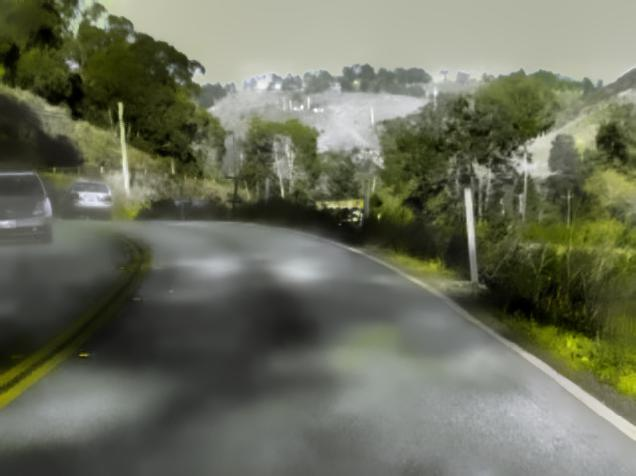
\includegraphics[width=.23\textwidth]{fps/rain}}
    \subfigure[]{\includegraphics[width=.23\textwidth]{fps/snow}}
    \subfigure[官方实验样例图]{
        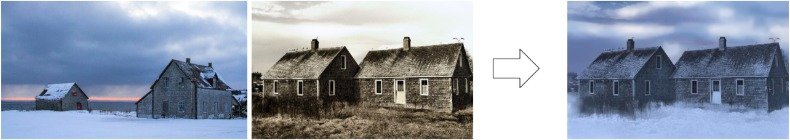
\includegraphics[width=.85\textwidth]{fps_o_1}
    }
    \caption{Fast Photo Style实验结果样例图}
    \label{fps-result}
\end{figure}

实际实现中,该算法官方给出了一个提前训练好的模型,其编码器$\varepsilon$使用了VGG-19网络结构中的conv1-1到conv4-1层,其权值由用ImageNet提前训练好的权值给定。训练数据集使用了微软COCO数据集\cite{coco}。总体来说,Fast Photo Style是一个能够实现快速合成真实图片风格转换的技术,它主要由格式化步骤和真实光滑化(photorealistic smoothing)步骤组成。该算法对上述两个步骤都给出了有效地闭环解决方案。

我们使用该模型进行了雨天、网上和雪天场景的转换,图\ref{fps-result}展示了最终实验结果样例图以及Fast Photo Style官方图像风格转换实验样例图。

% wc ~ 1000
% fast photo style要求content和style image内容尽可能相近

\subsubsection{Fast Neural Transfer}

\textbf{Fast Neural Transfer.}\cite{FNT} 该算法计算单个像素的损失函数时不止考虑低层级的像素信息,还利用损失网络中的高层级特征表示的感知损失函数来训练算法的网络结构。训练过程中,感知损失能够比单个像素损失函数更好的测量出图像之间的相似度。除了图像风格的转换,Fast Neural Transfer还可用于图像的分辨率升级等应用。它通过利用感知损失函数训练的前向转换神经网络将前向图像转换任务和优化后的图像合成技术结合了起来。

\begin{figure}[!bh]
    \centering
    \subfigure[]{\includegraphics[width=.23\textwidth]{FNT/origin}}
    \subfigure[]{\includegraphics[width=.23\textwidth]{FNT/night}}
    \subfigure[]{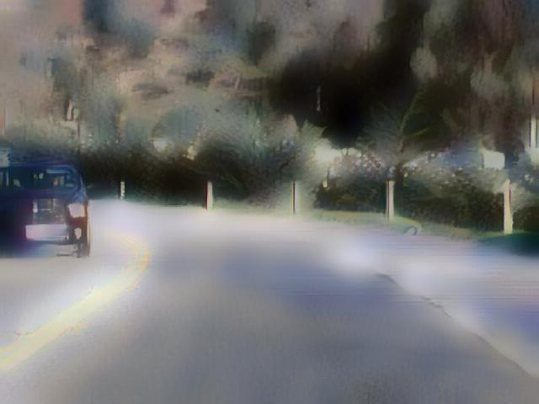
\includegraphics[width=.23\textwidth]{FNT/fog}}
    \subfigure[]{\includegraphics[width=.23\textwidth]{FNT/snow}}
    \subfigure[官方实验样例图]{
        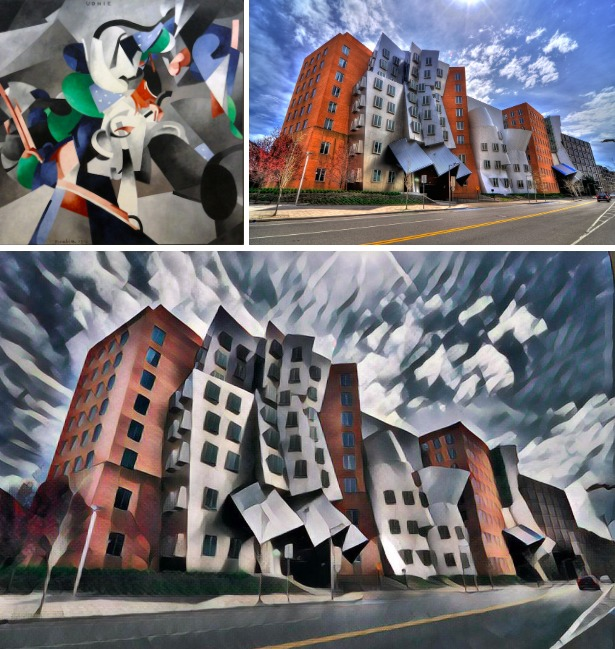
\includegraphics[width=.75\textwidth]{fnt_o_1}
    }
    \caption{Fast Neural Transfer实验结果样例图}
    \label{fnt-result}
\end{figure}

该算法系统由两部分:图像转换网络$f_w$和损失网络$\Theta$。其中损失网络用来定义多个损失函数$\ell_1,\dots,\ell_k$。图像转换网络是一个由权值$W$参数化的深度残差卷积神经网络。它通过映射函数$\hat{y}=f_W(x)$将输入图片$x$转换成输出图片$\hat{y}$。每个损失函数都会计算一个标量值$\ell_i(\hat{y},y_i)$来测量输出图片$\hat{y}$和目标图片$y_i$之间的距离。该图像转换网络的训练使用了一个复杂的梯度下降算法来最小化损失函数的权值组合:
\begin{align}
    W^*=\arg \min_W E_{x,\{y_i\}}\Big[\sum_{i=1}\lambda_i\ell_i(f_W(x),y_i)\Big]
\end{align}

为了解决单个像素损失的缺点,且是损失函数更好的测量出不同图像间的语义距离,该算法使用了提前为图像分类训练好的模型。因为这些模型一般都是卷积神经网络,且都在训练阶段学习了将我们想在损失函数中测量的语义信息编码的能力。因此,算法中为了定义损失函数,选择利用提前为图像分类训练好的网络模型$\Theta$作为固定的损失网络。

对于样式转换器,其输入和输出都是像素形状为$3\times 256 \times 256$的彩色图片。对于采样因子为$f$的高清图片,其输出是像素形状为$3\times288\times288$,输入为$3\times288/f\times288/f$。因为图像转换网络是全卷积的,所以在测试阶段它们可以用于任意分辨率的图片上。

算法中提出特征重建损失值是不同特征空间中的欧几里得距离:
\begin{align}
    \ell_{feat}^{\Theta,j}(\hat{y},y)=\frac{1}{C_jH_jW_j}||\Theta_j(\hat{y})-\Theta_j(y)||_2^2
\end{align}
当输出图片与目标图片的内容差异时特征重建损失函数会惩罚输出图片,对于输入$x$,网络$\Theta$中第$j$层的激活函数记为$\Theta_j(x)$,该函数是形状为$C_j\times H_j\times W_j$的特征图谱,定义Gram矩阵为$C_j\times C_j$的方阵,其元素有下面的公式给定
\begin{align}
    G_j^{\Theta}(x)_{c,\hat{c}}=\frac{1}{C_jH_jW_j}\sum_{h=1}^{H_j}\sum_{w=1}^{W_j}\Theta_j(x)_{h,w,c}\Theta_j(x)_{h,w,\hat{c}}
\end{align}

除此之外,该算法还定义了一个简单的损失函数:像素损失函数是输出图片$\hat{y}$和目标图片$y$间的欧氏距离。如果两者的尺寸形状都为$C\times H\times W$则像素损失为$\ell_{pixel}(\hat(y),y)=||\hat{y}-y||_2^2/CHW$。图\ref{fnt-result}为该算法在我们的数据集上实验的结果样例图以及Fast Neural Transfer官方的实验结果样例图。 

\subsubsection{UDPIR} 

\newmodel{UDPIR} 该算法的主要改进点在于它提出图像逆反表示的一种方法,该方法只利用图像表征的信息,以随机噪声图片为初始值,从而可以只包含表征自身的数据信息。图像的逆反表征问题本质上是寻找一张表征与给定图像最为接近和匹配的图片,即给定表征函数$\Phi:\mathbb{R}^{H\times W\times C}\to \mathbb{R}^d$和逆反表征$\Phi_=\Phi(x_0)$,图像可通过最小化下面的目标函数实现重建:
\begin{align}
    x^*=\min_x\in \mathbb{R}^{H\times W\times C}\mathb{l}(\Phi(x),\Phi_0)+\lambda\mathb{R}(x)
\end{align}
此处的$\mathb{l}$表示重建图像的表征与给定图像表征之间的距离,文献中具体的函数使用里欧几里得距离函数:
\begin{align}
    \mathb{l}(\Phi(x),\Phi_0)=||\Phi(x)-\Phi_0||^2
\end{align}
算法的具体实现中,依然采用了提前训练好的VGG19卷积神经网络的结构来重建图像,由于文献中没有给出官方的实验代码,我们依照文献中的方法复现了MNIST数据集中数字图像的重建,但是后面试图对路况图像进行重建实验中我们发现,该算法对于数据集中$256\times 256$图片的重建合成耗时过长,约2小时一张,效率过低,因此我们放弃了对该模型的进一步实验。

\subsubsection{Targeted Style Transfer}

\newmodel{Targeted-Style-Transfer} 该算法不同之处在于只修改目标图像的某一部分而不是全部,比如只修改图片中的某一个物体而不改变物体的背景和周围场景。算法实现中除了使用了基于深度神经网络的图片修改技术还需要图像语义分割技术的协助,在物体边界的光滑化和去锯齿化中使用了马尔可夫随机场模型。

算法的具体实现是基于Gatys提出的图像风格转换技术\cite{nst},给定包含了指定风格的原图片$s$,和目标转换图片$t$,算法目标是将图像$x$转换到风格与$t$类似的新图像中,但是其中的纹理信息保留。以上可以用下面的最小方差函数表示:
\begin{align}
    \min_x ||F(x)-F(t)||^2+||C(x)-C(s)||^2
\end{align}
$F(\cdot)$是将图像映射到对应的深度特征空间的映射函数,$C(\cdot)$是将图像映射到对应特征空间协方差的映射函数。

下图\ref{fig:tst}是Targeted Style Transfer的实验样例图,在实现我们的路况图像风格转换实验中,由于我们的需求往往是对道路或者天气的像素风格转换,而且转换后㛑需要对整个图像的整体风格也要做相应的调整,从而使得合成图像尽可能的真实。这使得我们需要对原始图片做大量的语义分割工作,而目前还没有专门这对这类工作的自动化流程代码出现,这使得我们要对整个路况图像库坐语义分割的预处理变得成本巨大,导致难以实现,因此我们也放弃了对该模型的进一步实验。 

\begin{figure}[h]
    \centering
    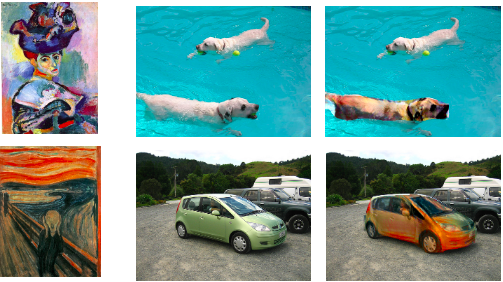
\includegraphics[width=.8\textwidth]{results/tst}
    \caption{Targeted Style Transfer实验样例图片}
    \label{fig:tst}
\end{figure}

\subsubsection{Feedforward style transfer}

\newmodel{Feedforward-style-transfer} 该算法对于图像转换任务使用了前向转换网络,与其他算法不同的是,其损失函数不是依靠图像中的低级信息,即每个像素之间的距离,而是使用图像中的高级特征之间的距离,即感知器损失函数。模型训练过程中,感知器损失函数对图像之间的差异度量比像素见的损失函数更加可信。

该模型的主要优点是在与其他图像风格转换算法取得相似效果的同时,其模型的训练更高效。其模型训练中使用的损失函数也是创新点所在,具体训练过程使用了stochastic梯度下降算法,其损失函数为:
\begin{align}
    W^*=\min_W\mathb{E}_{x,\{y_i\}}[\sum_{i=1}\lambda_il_i(f_W(x),y_i)]
\end{align}

由于该算法跟其他的图像转换技术算法一样,主要用于艺术画的图像合成,其实验结果样例图\ref{fig:fst}如下,所以我们将该算法用在路况图像转换上,最后的合成的路况图片也都太过艺术画了,与真实场景的驾驶路况场景差距太大,因此我们放弃了该模型的进一步实验数据统计和总结。 

\begin{figure}[h]
    \centering
    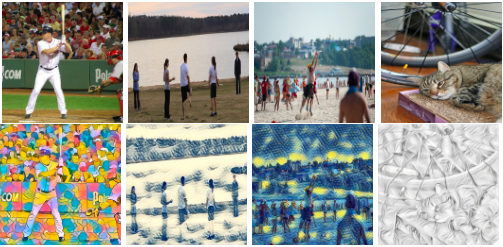
\includegraphics[width=.8\textwidth]{results/fst}
    \caption{Feedforward style transfer实验结果样例图}
    \label{fig:fst}
\end{figure}

% wc ~ 800

\subsubsection{Texture Nets}

\textbf{Texture Nets.}\cite{texture-nets}\quad 使用了前向生成网络来实现图像合成和风格化功能。该算法主要针对图像的纹理风格转换,文献\cite{texture-nets}中指出图片的纹理数据分布可由样本纹理数据$x_0$推导出,比如$x\sim p(x|x_0)$。在风格迁移中,分布是由图像$x_0$的视觉样式表征和另一张图片$x_1$的视觉内容表征推导出。特别的,为了从样本图片$x_0$合成纹理,这个问题可以表示为:
\begin{align}
    \min_{x\in \chi}||\Phi(x)-\Phi(x_0)||_x^2
\end{align}
对图像纹理来说,一般会假设$p(x)$是一个静态马尔科夫随机链。纹理$x_0$可以通以下公式估算局部区域的平均统计特征值:
\begin{align}
    \phi(x_0)=\frac{1}{|\Omega|}\sum_{i=1}^{|\Omega|}\psi_oF(x_0;i)\approx E_{x\sim p(x)}[\phi_oF_l(x;0)]
\end{align}

\begin{figure}[b]
    \centering
    \subfigure[]{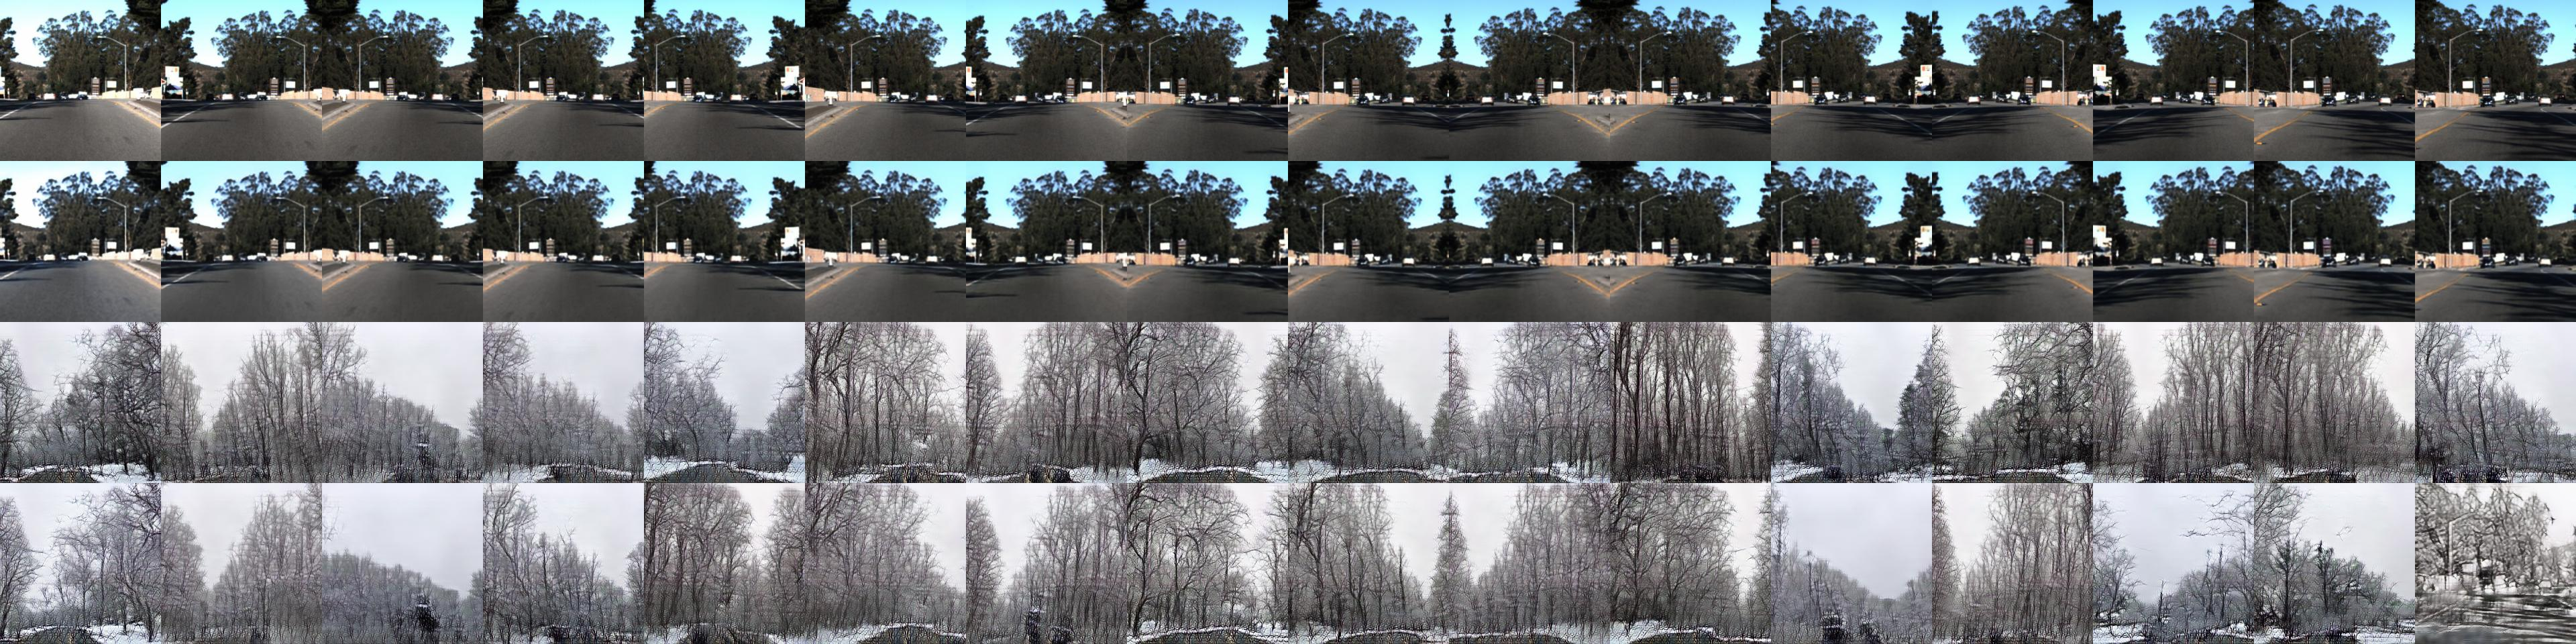
\includegraphics[width=.45\textwidth]{texture-nets/1}}
    \subfigure[]{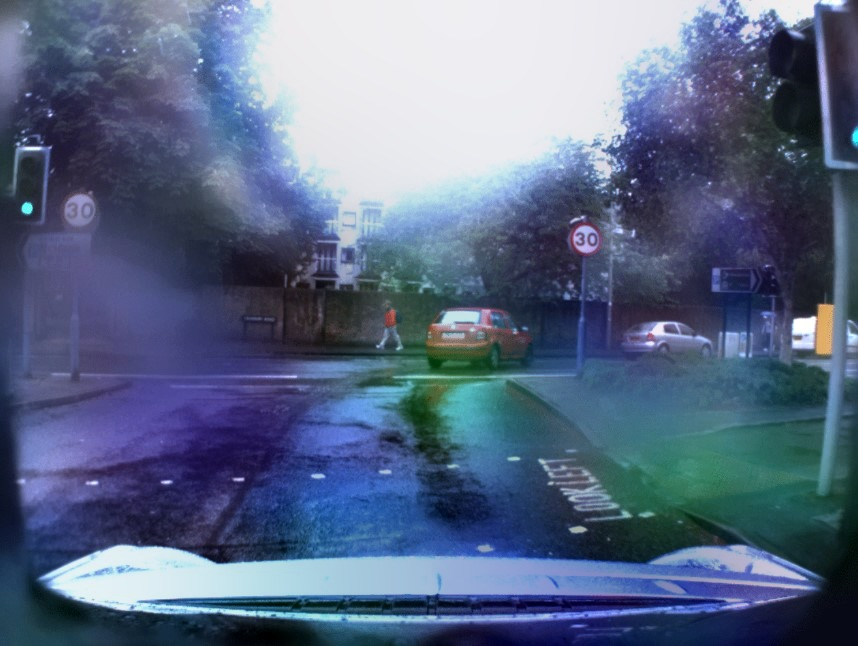
\includegraphics[width=.45\textwidth]{texture-nets/2}}
    \subfigure[官方实验样例图]{
        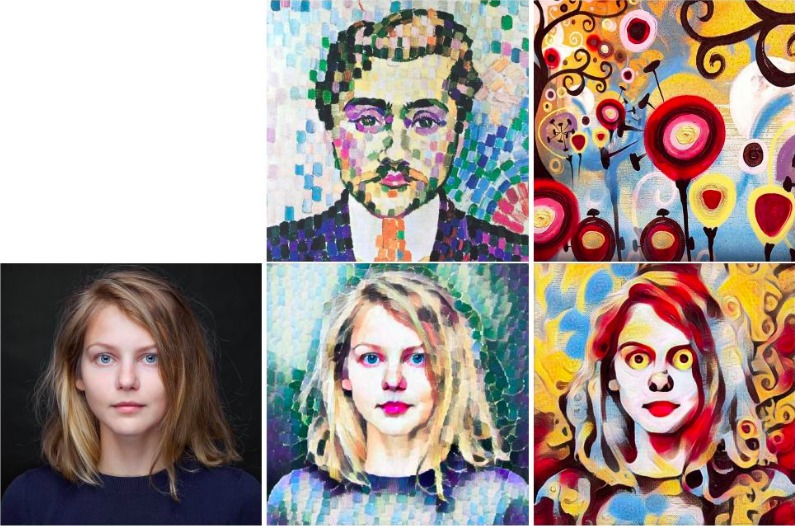
\includegraphics[width=.7\textwidth]{tn_o_1}
    }
    \caption{Texture Nets实验结果样例图} 
    \label{tn-example}
\end{figure}

同其他的图像风格转换技术类似,该算法的损失函数也是从文献\cite{nst}中推导出来的,图像的统计数据通过固定的提前训练好的卷积神经网络(通常是VGG网络)提取出来。其Gram矩阵可以定义成一个向量矩阵和特征图谱的点积:
\begin{align}
    G_{ij}^l(x)=<F_I^l(x),F_j^l(x)>
\end{align}
因为网络属性是卷积的,所以每个点积都是所有空间特征$i$和$j$激活函数的乘积之和。模型在实际训练过程中,将Gram矩阵$G^l,l\in L_T$组合用作纹理描述表征体,这里的$L_T$包含了表征体卷积网络中卷积层的下标指数。以上可以推导除下面的图像$x$和$x_0$之间的纹理损失:
\begin{align}
    L_T(x;x_0)=\sum_{l\in L_Y}||G^l(x)-G^l(x_0)||_2^2
\end{align}
除了纹理损失函数,该算法还提出基于卷基层$l\in L_C$的输出$F_i^l(x)$来比较图片差异:
\begin{align}
    L_C(x;y)=\sum_{l\in L_C}\sum_{i=1}^{N_t}||F_i^l(x)-F_i^l(y)||_2^2
\end{align}
这里的$N_t$是第$l$层的特征通道个数。与纹理损失的主要差别在于内容损失在对应的空间区域比较特征激活函数,因此保留了空间位置信息。因此内容损失函数对于内容信息保留来说更合适,但对于纹理信息去并不合适。

算法中具体的学习过程是通过调整生成器$g(y_i,z_i;\theta)$参数$\theta$来最小化内容和纹理损失函数的组合值:
\begin{align}
    \theta_{x_o}=\min_{\theta}E_{z\sim Z;y\sim Y}[L_T(g(y,z;\theta),x_0)+\alpha L_C(g(y,z;\theta),y)]
\end{align}
这里的$Z$表示纹理合成图片的噪声分布,$y$是真实图片的实际分布,$\alpha$是平衡纹理/样式和内容的参数。图\ref{tn-example}为该模型的最终实验结果样例图以及Texture Nets官方实验结果样例图。


\section{本章小结}

本章主要介绍了该实证研究项目的实验方法设计:即实验数据比较指标的设计,实验比较模型的筛选历程,以及对选取的每个模型进行了简要的原理介绍。在模型筛选过程中本实验初期进行了大量的实验,由前文介绍的,最终由于种种原因:源码未开放,无法针对每个技术模型收集到最匹配的训练数据集,合成图与我们路况天气风格转换与合成的需求有较大出入等原因进行了大量的取舍,最终记录在论文中的是我们重点实验过的模型,参与实验最后数据的统计与比较的一共有8个DNN模型,主要为对抗生成网络和图像风格转换迁移技术。

此外所有的实验都是在Ubuntu 16.04 LTS操作系统,8核GeForce GPU的计算机上进行的,所有的合成图像数据统一使用Python pickle包压缩后存储于MySQL数据库中,未来计划开源在GitHub上。

% wc ~ 800

